A wind farm is a collection of wind turbines in a single location. It collects the energy from the wind and extracts wind power. Due to the increasing price of energy, the number of wind farms around the globe also increases. Unfortunately, installation of wind farms does not always come in handy. It leads to most common con of wind farm, that is the extracted energy from the wind is not maximized, thus causing the wind farm to be unreliable and inefficient \cite{windturbine1}.

In wind farms, there is a phenomenon which causes the decrease of the extracted energy from the wind. It is called the \textbf{Wake Effect}. The wind through the downstream wind turbine is significantly slower than the wind through the upstream wind turbine. Basically, the wind leaving a turbine is slowed down thus the energy extracted by the downstream turbine is lower than the upstream turbine \cite{wakeeffect}. Finding the best location for each turbine in a wind farm helps prevent the wake effect, thus increases effectiveness. This is called \textbf{wind turbine siting}.

The aim of this study \cite{this} is to show a solution that can help minimize the wake effect. The position of each individual turbines with respect to other turbines will affect the wake. To simulate the wind farm, Jensen's Wake Model \cite{book2} is used along with the Sum of Squares Method, to determine the wind speed through each wind turbine. A genetic algorithm based local search was used to show a solution to the problem.

Wind turbines are devices that produce energy from the wind to electricity. It uses the kinetic energy from the wind and convert it to electric energy. The blades of the wind turbines rotate at 13 - 20 rounds per minutes (RPM) though it depends on different wind turbines \cite{windturbine2}. Depending on the velocity of the wind in locale, the wind turbines can convert energy varies every day.

Wind turbines structures have a general blueprint. Wind turbines have an anemometer and wind vane on the top. Wind vane determines which direction is the wind coming from while the anemometer determines the velocity of the wind. This helps maximize the energy converted by the wind turbines by getting the most out of the wind. Wind turbines can rotate in its axis to face where the wind is coming from using the Yaw drive connected to the Yaw motor. Each blades of the wind turbine can also turn to maximize resistance from the wind itself. Depending on the velocity of the wind, the wind turbine will stop spinning if the wind's velocity is too high for safety. The rotors of the wind turbine is connected to a low-speed shaft. This low-speed shaft turns in the same RPM as the rotors. The low-speed shaft is then connected and stored inside a gearbox with the high-speed shaft and connects them together. This gearbox multiplies the RPM of the low-speed shaft to about hundred times for the high-speed shaft. The high-speed shaft is connected to a generator that produces electricity using the kinetic energy of the rotations of the high-speed shaft. All of this components are installed inside the nacelle. A nacelle is the container located at the top of the turbine tower and connects the blades and the tower. The electricity then flows through the interior of the tower of the wind turbine to the base where the transformer is. The transformer converts the electricity to alternating current which is then connected to the substations via underground cables. The substations then distributes the electricity to the power grid and then travels to the public to use \cite{windturbine3}.
\begin{figure}
            \centering
            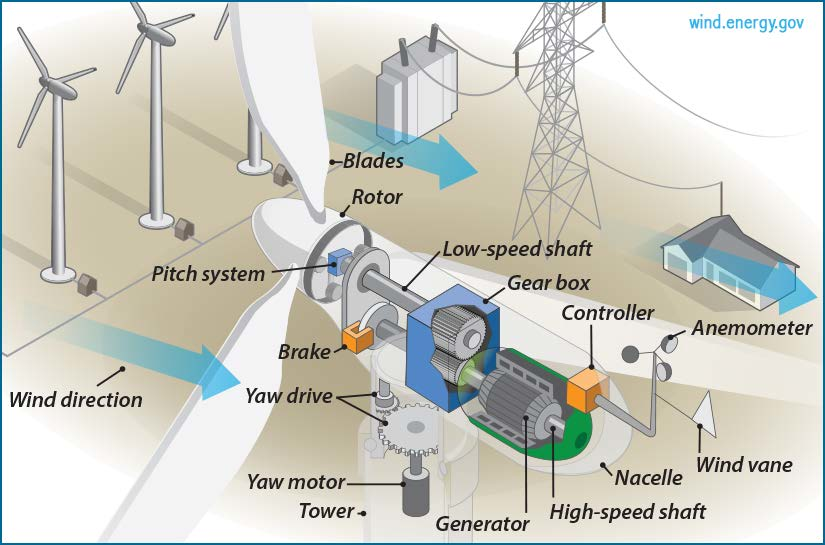
\includegraphics[width=130mm, height = 80mm]{Figures/windMotor.png}
            \caption{Parts of the Wind Turbine \cite{windPrt}}
            \label{fig:my_label}
\end{figure}